%%%%%%%%%%%%%%%%%%%%% chapter.tex %%%%%%%%%%%%%%%%%%%%%%%%%%%%%%%%%
%
% Capítulo Introdução ao Intel Galileo
%
% Laboratório 0: Como fazer um LED piscar
%
%%%%%%%%%%%%%%%%%%%%%%%% Springer-Verlag %%%%%%%%%%%%%%%%%%%%%%%%%%
\chapter{Introdução ao Intel Galileo}
\label{intro} % Always give a unique label
% use \chaptermark{}
% to alter or adjust the chapter heading in the running head

\abstract{O objetivo deste capítulo é introduzir os principais fundamentos da placa Intel Galileo e apresentar as ferramentas e componentes necessários para o início do desenvolvimento de projetos com a mesma. Também será desenvolvido o primeiro projeto utilizando a placa: Como fazer um LED piscar.}

\section{A placa Intel Galileo}
\label{sec:1}

A placa Intel Galileo (Figura 1.1) é uma placa de desenvolvimento certificada em Arduino baseada na arquitetura Intel x86 utilizada para fins tanto educativos quanto comerciais. A placa necessita de uma fonte de 5V e, quando ligada via usb num computador, pode ser programada através de sistemas Windows, Linux e Mac OS pois suporta a IDE Arduino, que é compatível com esses sistemas. Assim, para iniciar o desenvolvimento com a placa é necessário que seja instalado no computador o driver específico da placa e a IDE Arduino. 
Observação: para evitar possíveis danos aos componentes da placa, recomenda-se ligar a mesma a fonte primeiro e depois ao usb do computador. 

\begin{figure}[h]
\centering
\includegraphics[scale=0.3]{chapter1/galileo.jpg}
\caption{Placa Intel Galileo}
\label{fig:1}
\end{figure}

\section{Software}
\label{sec:2}

Para o desenvolvimento dos laboratórios será utilizado o software do ambiente de desenvolvimento (IDE) Arduino (Figura 1.2), o software pode ser facilmente encontrado para livre download na internet e, uma vez baixado, pode rodar diretamente em qualquer um dos sistemas Windows, Linux e Mac OS pois é um aplicativo feito em Java. Após a instalação do driver da placa, realiza-se a configuração da IDE onde deve-se selecionar no menu ferramentas (Figura 1.3) a placa utilizada, no caso Intel Galileo, e a porta na qual a mesma está conectada, uma usb do computador. Com todas as configurações prontas podemos conectar a placa ao computador, fazer as conexões com os pinos da placa e tranferir para a mesma o código compilado pela IDE.

\begin{figure}[h]
\centering
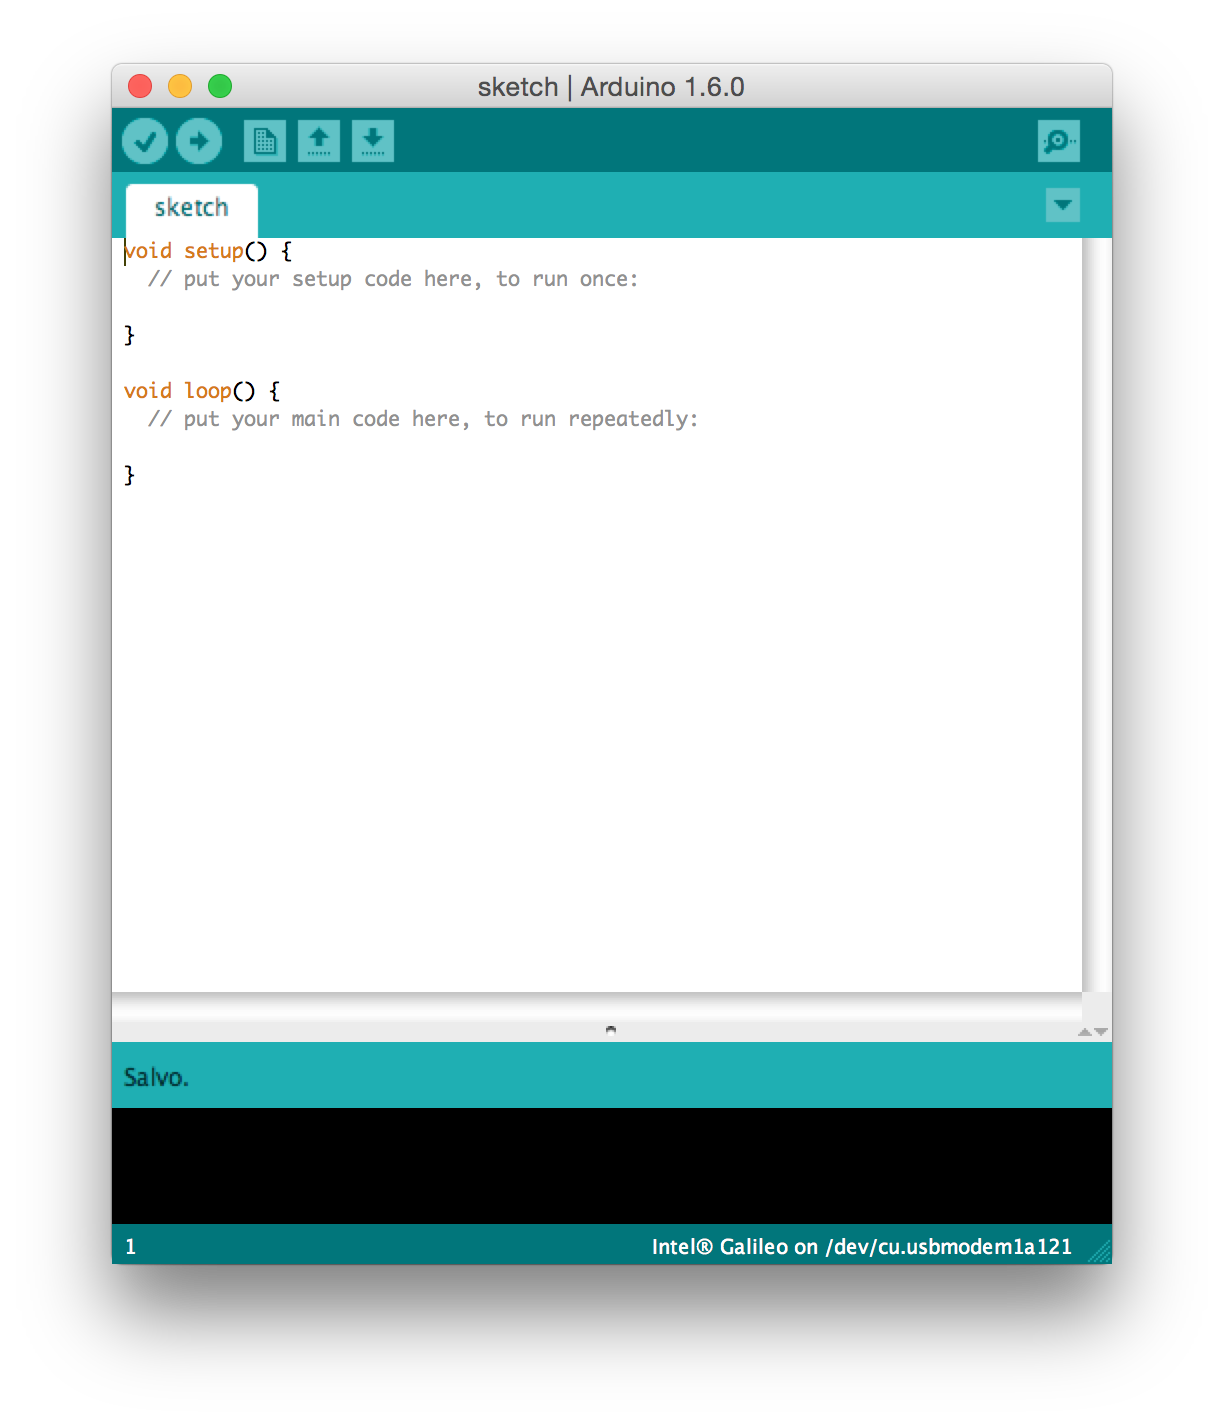
\includegraphics[scale=0.5]{chapter1/IDE1.png}
\caption{IDE Arduíno}
\label{fig:2}
\end{figure}

\begin{figure}[h]
\centering
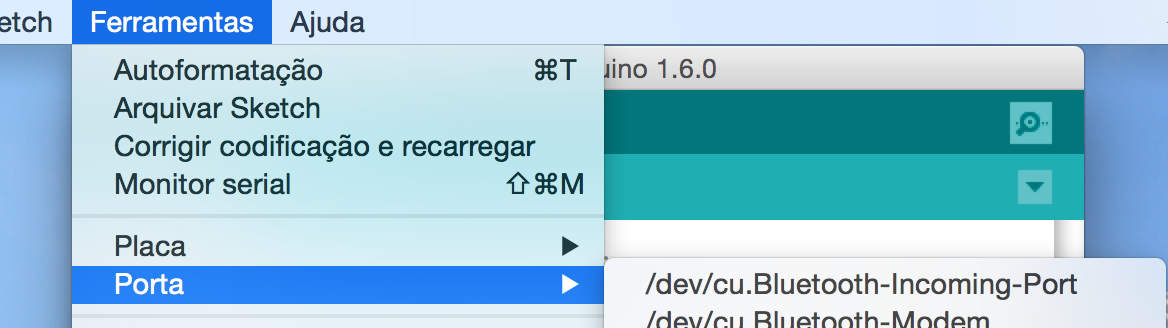
\includegraphics[scale=0.6]{chapter1/IDE3.png}
\caption{Seleção da placa e da porta}
\label{fig:3}
\end{figure}

\section{Componentes}
\label{sec:3}

Para a realização dos laboratórios, alguns componentes eletrônicos serão necessários, a seguir serão apresentados alguns deles

\subsection{Resistor}
\label{subsec:1}
Utilizado para limitar a corrente elétrica que passa por um determinado ponto do circuito, o resistor (Figura 1.4) é de extrema importância pois além servir como componente auxiliar, ele pode ser considerado também um componente de segurança, pois em determinadas situações, ao limitar a corrente no circuito, ele impede que ocorra dano a um outro componente que não suporta a corrente mais alta. Os resistores são identificados por cores, onde cada combinação de cor representa um valor para o resistor. Nos laboratórios a seguir serão utilizados principalmente os resistores de valor 330k$\Omega$ e 68$\Omega$.

\begin{figure}[h]
\centering
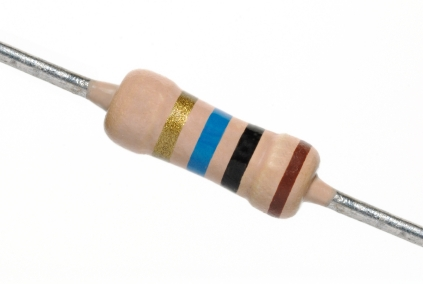
\includegraphics[scale=1.5]{chapter1/resistor.jpg}
\caption{Resistor}
\label{fig:4}
\end{figure}

\subsection{LED}
\label{subsec:2}
Um LED (Figura 1.5) emite luz quando excitado por pequena corrente elétrica, sendo que a corrente passa do pino mais longo do LED para o pino mais curto. Muito vezes deve ser utilizado com um resistor pois não suporta as altas tensões dos circuitos.

\begin{figure}[h]
\centering
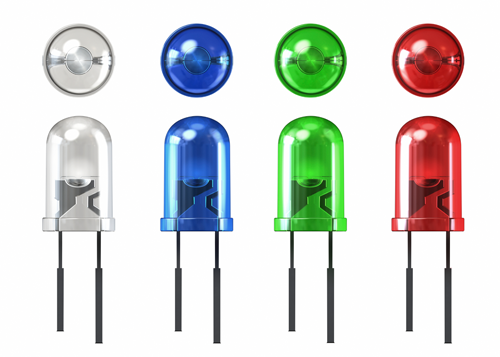
\includegraphics[scale=1.5]{chapter1/led.png}
\caption{LEDs}
\label{fig:5}
\end{figure}

\subsection{Chaves}
\label{subsec:3}
Algumas chaves serão utilizadas nos laboratórios, eles poderão ser dos tipos táctil (momentânea) (Figura 1.6), gangorra (Figura 1.8) ou tipo botão (Figura 1.7).

\begin{figure}[h]
\centering
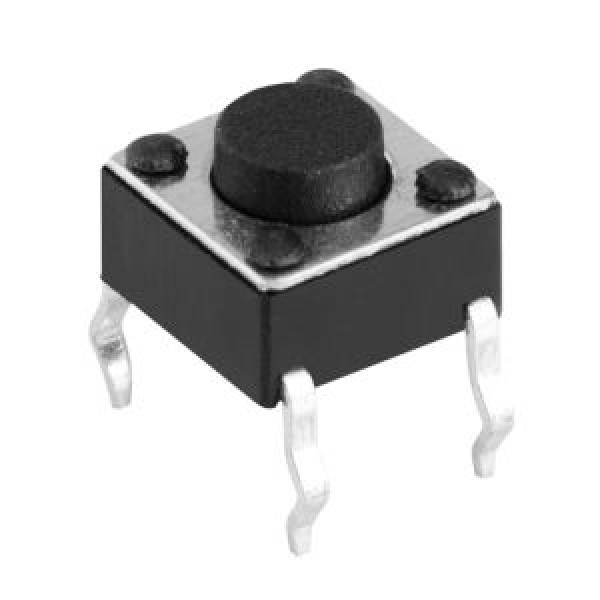
\includegraphics[scale=0.15]{chapter1/tactil.jpg}
\caption{Chave táctil}
\label{fig:6}
\end{figure}
\begin{figure}[h]
\centering
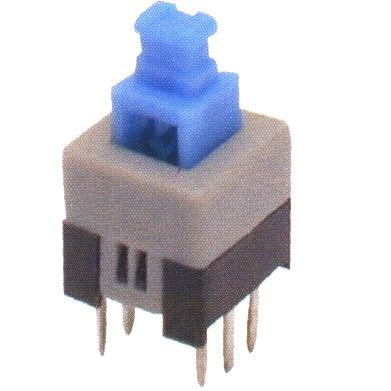
\includegraphics[scale=0.3]{chapter1/botao.jpg}
\caption{Chave tipo botão}
\label{fig:7}
\end{figure}
\begin{figure}[h]
\centering
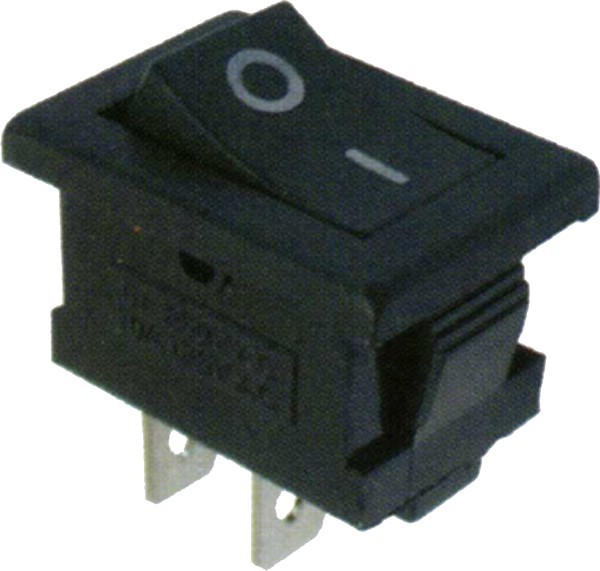
\includegraphics[scale=0.13]{chapter1/gangorra.jpg}
\caption{Chave gangorra}
\label{fig:8}
\end{figure}

\subsection{Sensores}
\label{subsec:3}
Dois tipos de sensores serão utilizados nos laboratórios, sensor de temperatura (Figura 1.9) e sensor de luminosidade (Figura 1.10).

\begin{figure}[h]
\centering
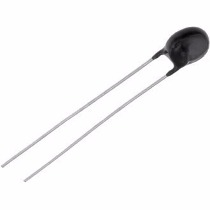
\includegraphics[scale=0.4]{chapter1/sensortemp.jpg}
\caption{Sensor de temperatura}
\label{fig:9}
\end{figure}
\begin{figure}[h]
\centering
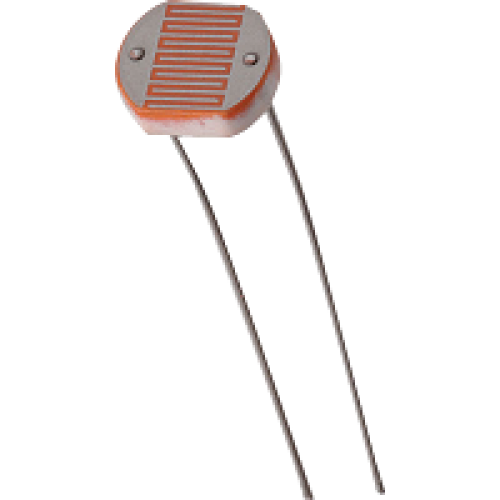
\includegraphics[scale=0.15]{chapter1/sensorlumi.png}
\caption{Sensor de luminosidade}
\label{fig:10}
\end{figure}

\subsection{Protoboard}
\label{subsec:4}
A protoboard (Figura 1.11) é uma placa auxiliar que possui conexões internas ligando os pequenos furos onde são conectados fios e componentes. Na Figura 1.12 temos as formas como os furos estão conectados no interior da protoboard.

\begin{figure}[h]
\centering
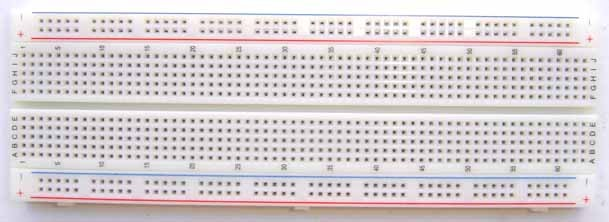
\includegraphics[scale=0.6]{chapter1/protoboard.jpg}
\caption{Protoboard}
\label{fig:11}
\end{figure}
\begin{figure}[h]
\centering
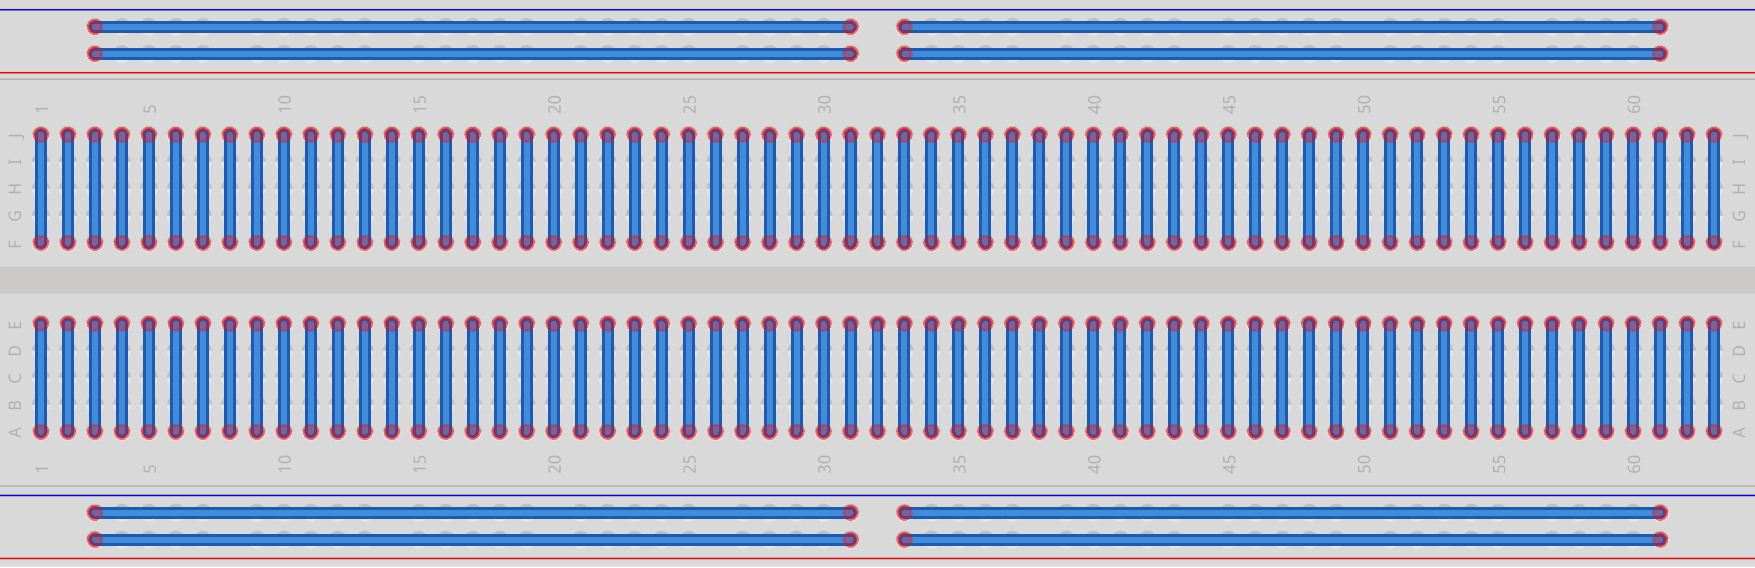
\includegraphics[scale=0.8]{chapter1/conexoes.jpg}
\caption{Conexões na protoboard}
\label{fig:12}
\end{figure}


\section{Laboratório 0}
\label{sec:4}
Para introduzir ao desenvolvimento com a placa Intel Galileo e o conceito de programação para Arduino, o primeiro laboratório será o mais básico: Como fazer um LED piscar. Neste labóratório o programa faz um LED piscar, ou seja, o LED permanece ligado por 1/2 segundo e depois desligado por 1/2 segundo, repetidamente. Para tal, primeiro deve-se montar o circuito à placa seguindo o diagrama da Figura 1.13 abaixo:
\begin{figure}[h]
\centering
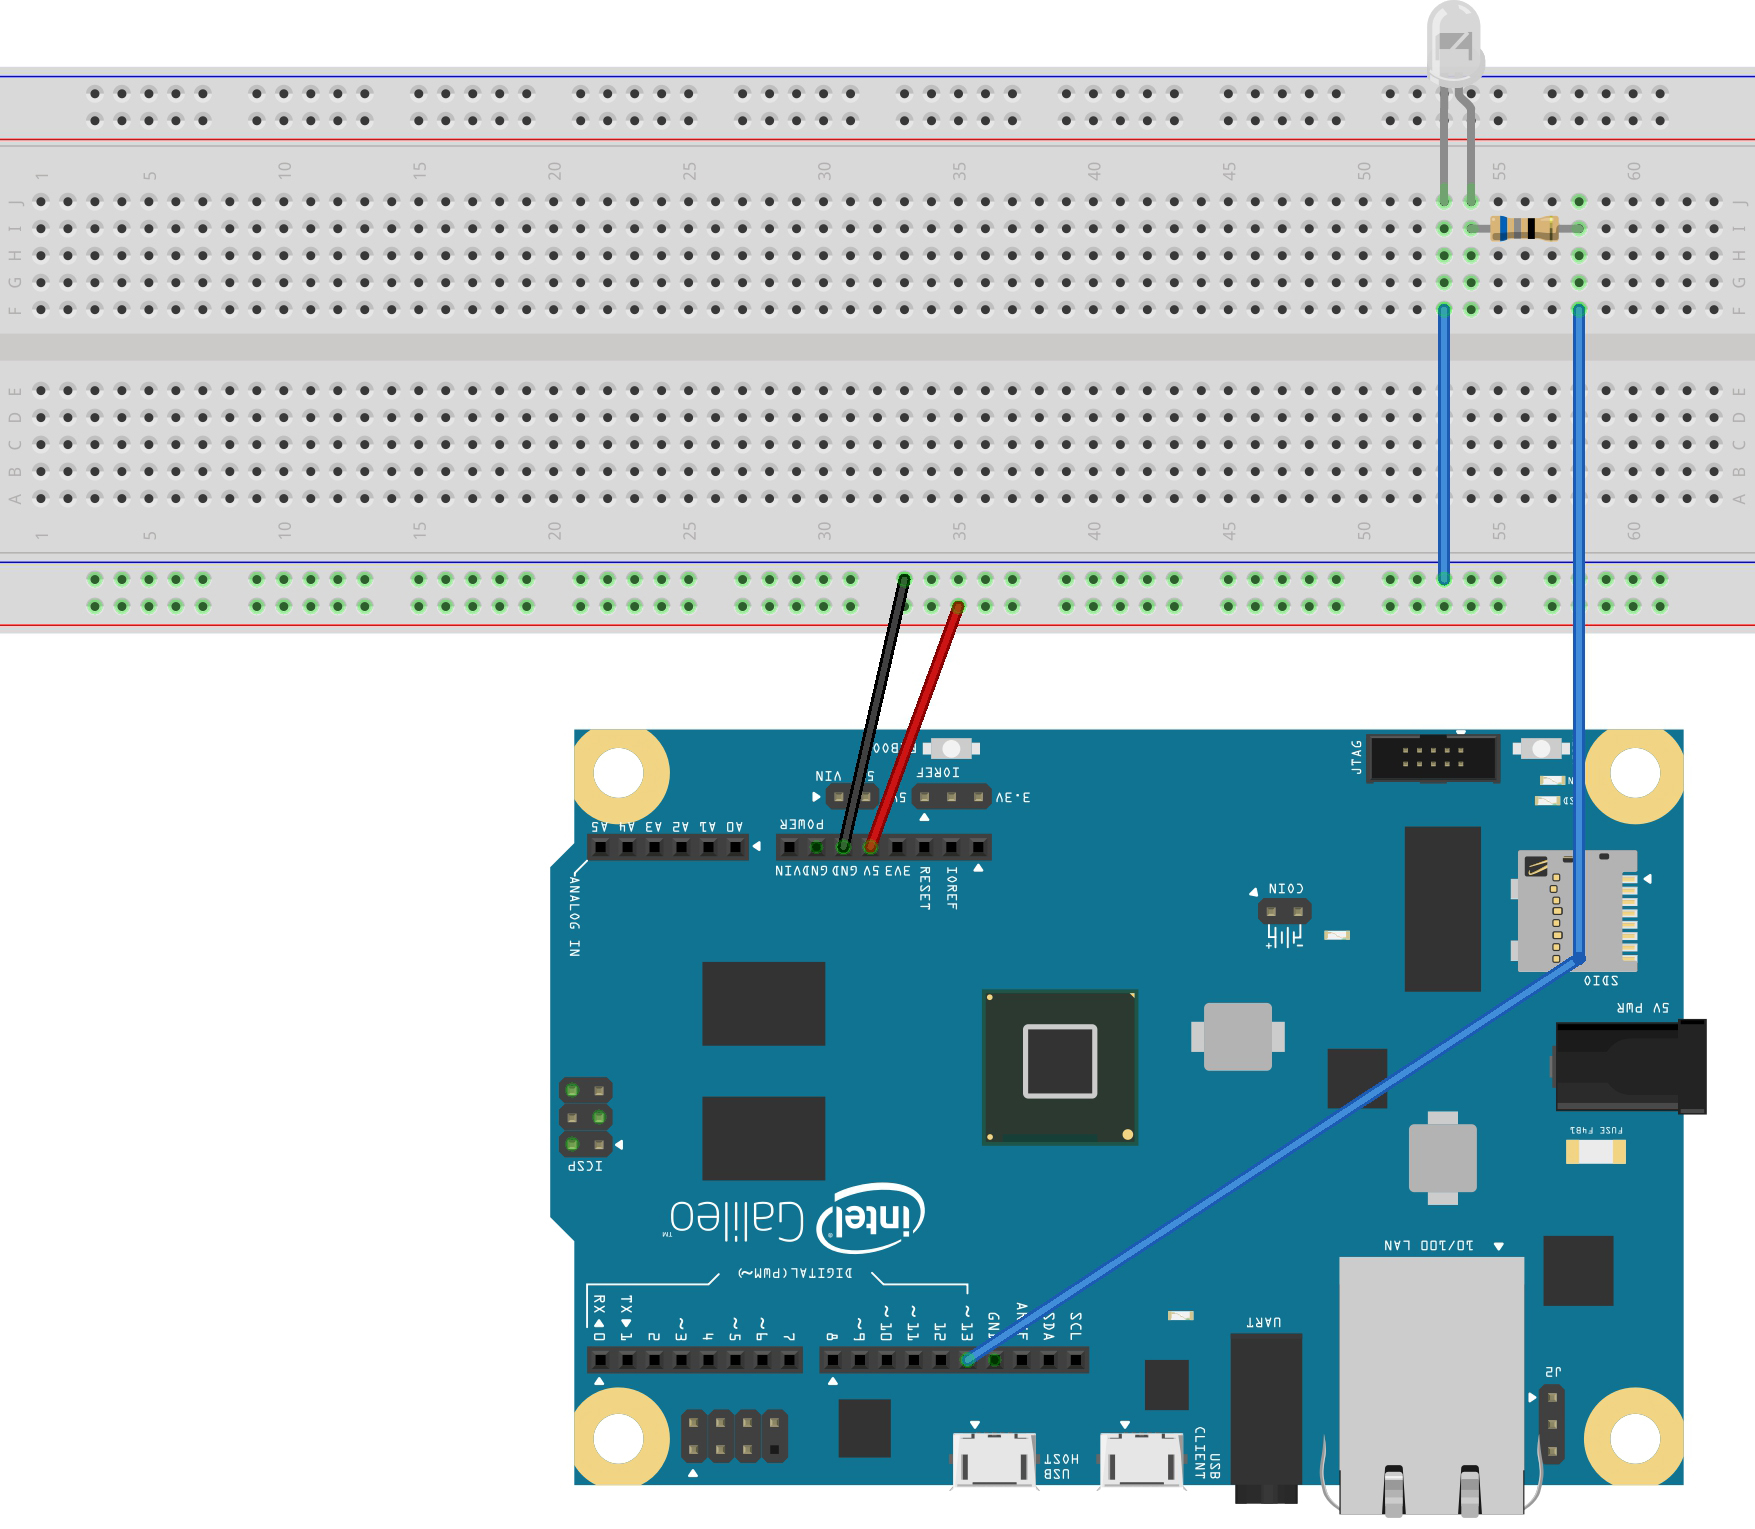
\includegraphics[scale=0.7]{chapter1/blink.jpg}
\caption{Diagrama do laboratório 0}
\label{fig:13}
\end{figure}

Após, passamos, através da IDE Arduino, o código (introducao.ino) abaixo para a placa e verificamos o acendimento do LED.

\lstinputlisting[float=h]{chapter1/introducao.ino}

Como pode-se observar no código acima, um programa para arduino é conhecido como sketch e todo sketch possui duas rotinas principais: setup() e loop(). A rotina setup(), é executada primeiro e apenas uma vez, ela é utilizada para a inicialização de variáveis, configuração dos pinos da placa e inserção de bibliotecas. Já a rotina loop() é executada logo em seguida e se trata de um laço que executará até o desligamento da placa ou a troca de programas, ele é utilizada para controle, ou seja, é onde se encontra a lógica do algoritmo. No código, a linha \textbf{int ledPin1 = 13;} identifica o pino, a linha \textbf{pinMode(ledPin1, OUTPUT);} configura o pino 13 da placa, que está conectado ao resistor e ao LED, como saída, as linhas \textbf{digitalWrite(ledPin1, HIGH);} e \textbf{digitalWrite(ledPin1, LOW);} acendem e apagam o LED e a linha \textbf{delay(500);} faz o programa esperar por 500ms ou 1/2 segundo. 